
\documentclass{sig-alternate-05-2015}


\begin{document}

% Copyright
\setcopyright{acmcopyright}

% DOI
%\doi{}

% ISBN
%\isbn{}

%Conference
%\conferenceinfo{}{}

%\acmPrice{}

%
% --- Author Metadata here ---
%\conferenceinfo{}{}
%\CopyrightYear{2007} % Allows default copyright year (20XX) to be over-ridden - IF NEED BE.
%\crdata{0-12345-67-8/90/01}  % Allows default copyright data (0-89791-88-6/97/05) to be over-ridden - IF NEED BE.
% --- End of Author Metadata ---

\title{Leveraging Spark and Docker for Scalable, Reproducible Analysis of Railroad Defects}

\numberofauthors{2}
\author{
% 1st. author
\alignauthor
Dylan Chapp\\
       \affaddr{University of Delaware}\\
       \email{dchapp@udel.edu}
% 2nd. author
\alignauthor
Surya Kasturi\\
       \affaddr{University of Delaware}\\
       \email{suryak@udel.edu}
}

\maketitle
\begin{abstract}
The resiliency of railroad networks depends on the ability of railroad 
engineers to identify and mitigate track and rail defects. As railroads
modernize their defect identification measures, the volume and velocity of 
defect data substantially increases, necessitating adoption of techniques
for ``Big Data" analytics. We present a study of railroad defect prediction 
built atop Apache Spark and Docker to achieve scalability and reproducibility.
\end{abstract}
%\keywords{}

\section{Introduction}
According to the United States Federal Railroad Administration Office of Safety Analysis, track defects are the second leading cause of accidents on railways in the United States.
In light of the economic significance of railway accidents~\cite{Schafer:08}, there is a pressing need in the railroad engineering community to adopt data-driven scalable data analysis tools from the greater ``Big Data" ecosystem.~\cite{Zarembski:14} 
Track maintenance--i.e., identifying and repairing defects--is one of the primary factors that affect the service life of a rail track, but due to the severe safety implications of undeftected or unrepaired defects, the ability to predict common defects is highly desirable. 

In this work, we present a case study centered on the analysis of two railroad defect data sets
obtained from railroad engineering researchers in the University of Delaware Department of 
Civil Engineering. Hereafter we will refer to these datasets as the \texttt{rail\_defects} data 
set and the \texttt{track\_geometry\_defects} data set. Respectively, these data sets describe 
defects in the rails themselves, such as voids or internal changes in crystalline structure, 
and misalignment of track components, such as one rail tilting away from the other.~\cite{Zarembski:14}
We investigate the feasibility of predicting the type of a defect based on associated data such 
as geographic region, mean gross tonnage (MGT) the track is subject to, and rail type. 
In the rest of this paper, we outline the construction of our analysis platform, present some
initial results on classification accuracy, and propose extensions to our work. 

\section{Methodology}
Both of the data sets we target have mixed categorical and numerical features and $>99\%$ of
the individual defect records have a class label indicating the type of defect. In the case of 
\texttt{rail\_defects}, there are 20 distinct defect types. For  
\texttt{track\_geometry\_defects}, there are 25 defect types. In light of these properties, we
focus on the multilabel classification task for each data set. We decompose the task into a 
pipeline of three parts: preprocessing, training, and testing. We implement this pipeline using
the MapReduce framework Apacahe Spark~\cite{Zaharia:2012} and its parallel machine learning library
MLLib, and package the data and analysis scripts as a Docker container for ease of dissemination. 
In the remainder of this section, we describe the pipeline components, also display in 
Figure~\ref{fig_block_diagram}
\begin{figure}[ht!]
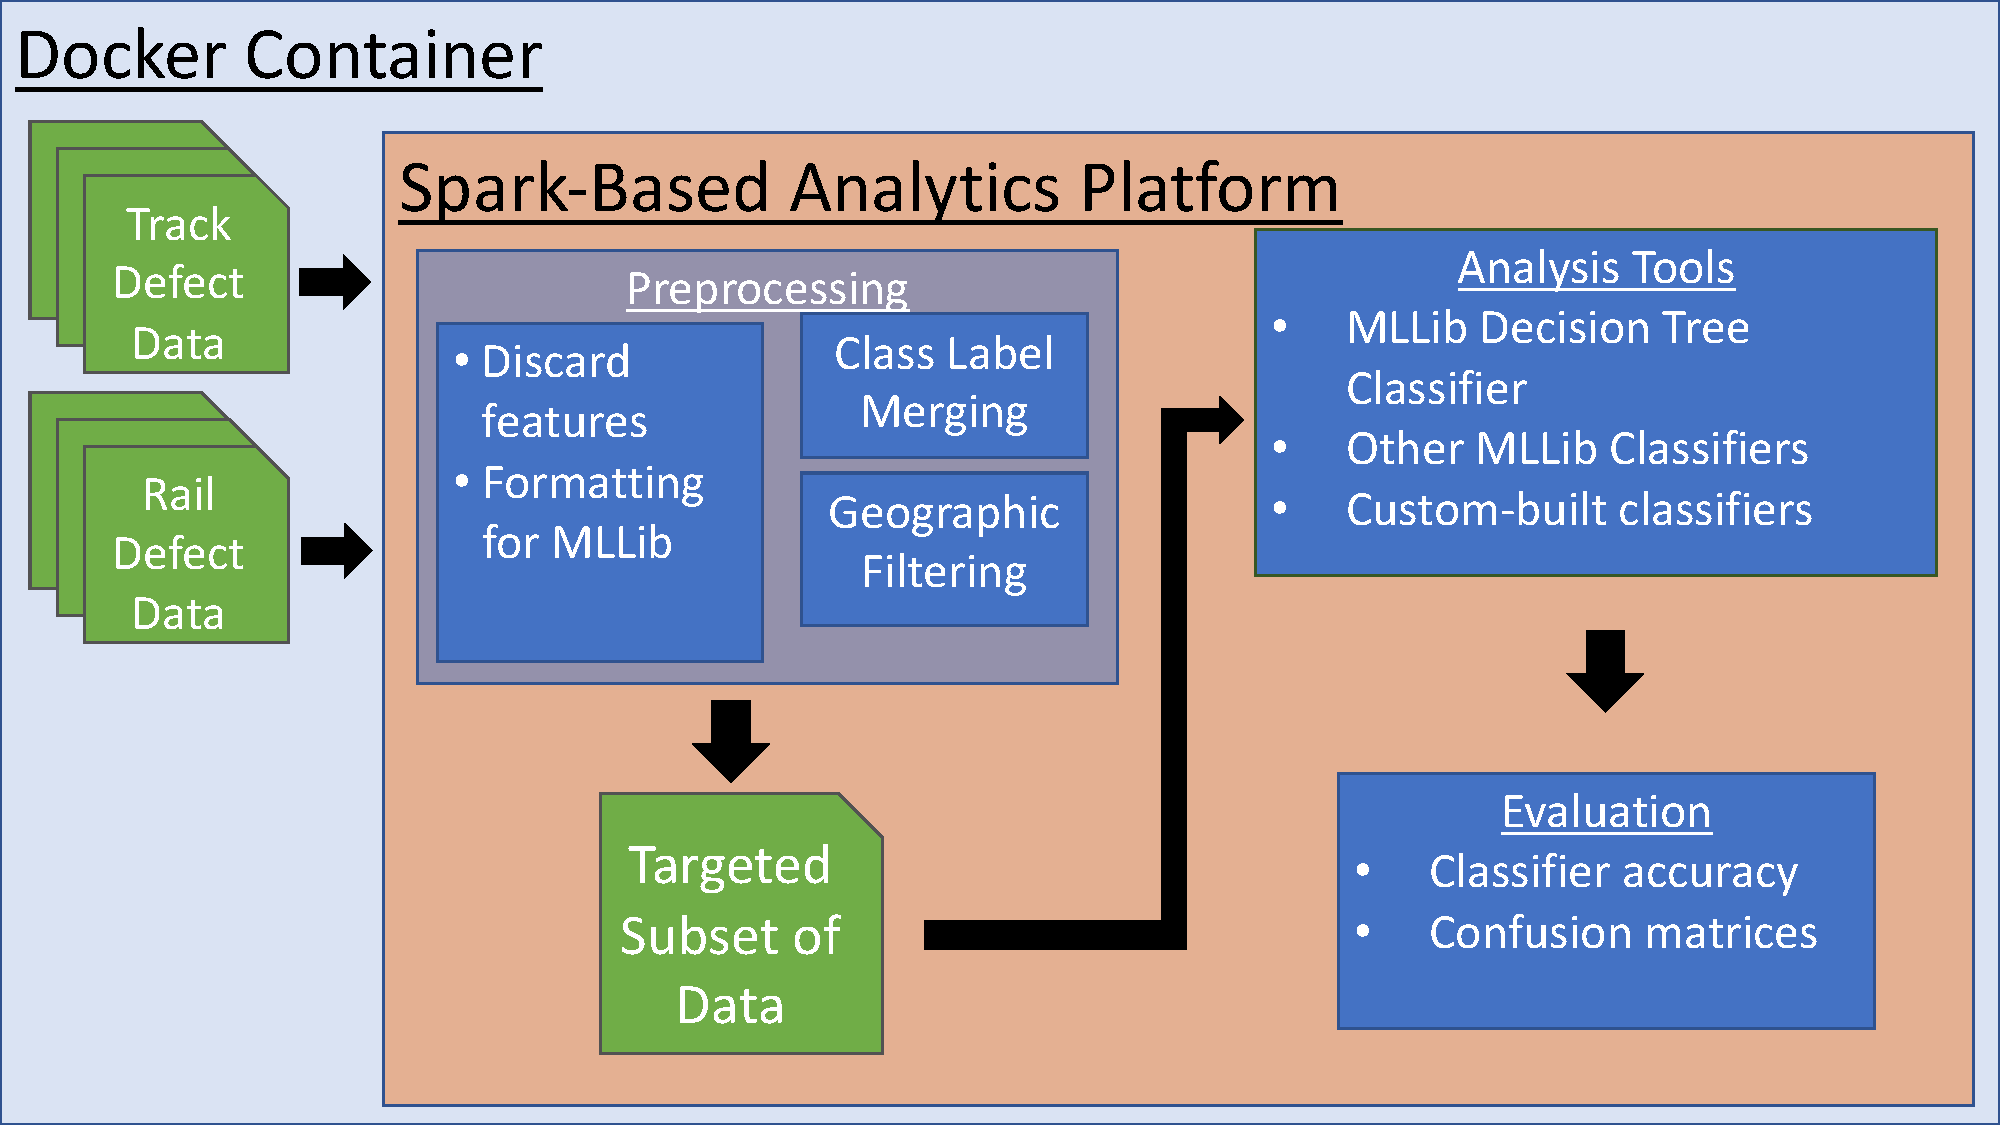
\includegraphics[width=0.50\textwidth]{block_diagram.pdf}
\caption{Block Diagram of Analytics Platform}
\label{fig_block_diagram}
\end{figure}

We consider two stages of mandatory preprocessing. The first stage discards all columns except 
for a specified set, then discards any rows that are missing values for features from that set. 
The second stage maps the raw record strings to the format the MLLib API specifies, a key-value 
pair whose key is the type of defect and whose value is a feature vector.In addition to the
above preprocessing, we implemented two optional stages: one to restrict the data to a 
geographically coherent region, and another to map each data point's class label to a ``super-
class" label indicating the general kind of defect (e.g., a welding-related defect, rather than 
one of the five kinds of specific welding defects). In our evaluation section, we demonstrate
the usefulness of these additional preprocessing stages. 

To build and evaluate our classifier, we split the subset of data remaining after preprocessing into
training and testing sets consisting of, respectively, $70\%$ and $30\%$ of the original data. 
Membership in the training and testing sets is determined by uniform random samplying. We then 
train an instance of MLLib's decision tree classifier on the training set and test its predictions.
In principle, any other MLLib classifier with a compatible API could be trained instead, but we 
elected to keep our classifier type fixed and investigate the effect of the ``class-merging" and 
``geographic filtering" preprocessing steps on accuracy. 



\section{Evaluation}
To evaluate our classifier's performance, we examine the overall accuracy rate of the classifier
and its associated confusion matrix. When we train the classifier on training data drawn 
uniformly at random from the 

\subsection{Class Label Merging}

\subsection{Geographic Filtering}
We propose that if subdivisions have similar numbers of each kind of defect, then we should
group these subdivisions' data points and train a classifier with the expressed purpose of 
achieving good accuracy for that set of subdivisions. To determine which subdivisions to merge,
we propose computing the $\chi$-squared distance $S$ defined below for each pair of 
subdivisions, then merge them based on a fixed threshold. 
\begin{center}
    $S(D_1,D_2) = \sum\limits_{i=0}^{N}\frac{(x_i - y_i)^2}{(x_i + y_i}$
\end{center}
We demonstrate the potential of grouping based on defect type distributions below. We compute
$S(x,y)$ for each pair of subdivisions within the Appalachian division and display the results
in the heat map in Figure~\ref{similarity_heatmap}
\begin{figure}[ht!]
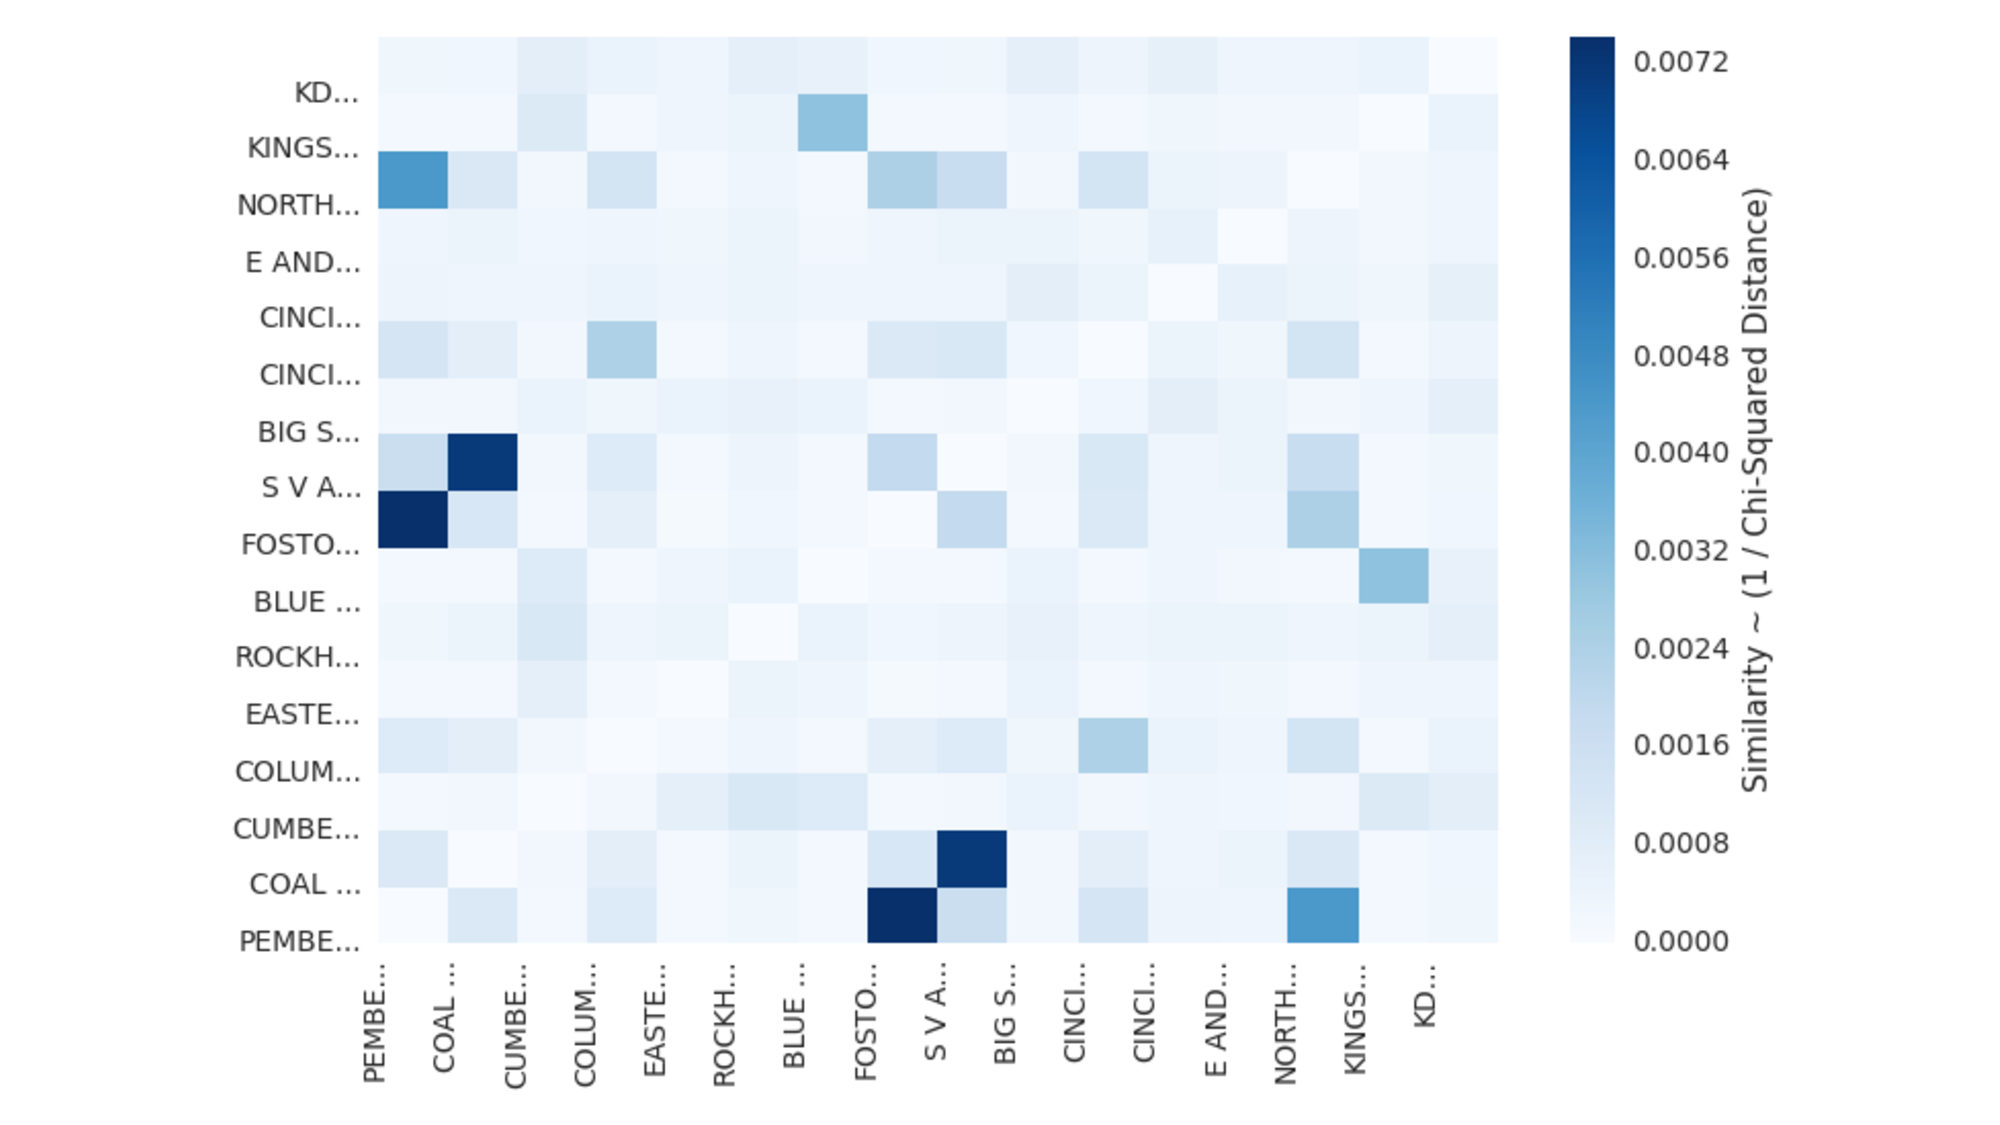
\includegraphics[width=0.5\textwidth]{similarity_heatmap.pdf}
\label{similarity_heatmap}
\caption{$\chi$-squared distance between defect distributions for each subdivision}
\end{figure}

\section{Conclusions and Continuing Work}
We identified the potential of a hierarchical classification stage to improve the accuracy of 
defect type predictions. Additionally, we determined while that merely training classifiers on 
data from geographically-similar regions does not yield a significant improvement in accuracy, 
attempting to group together regions whose defect distributions are similar may prove useful. 

Future directions for this work include evaluating classifiers beyond decision trees, and 
refining the similarity metric on defect distributions we use to group regions.



\bibliographystyle{abbrv}
\bibliography{bib}  
\end{document}


%However, we do not pursue any kind of unsupervised learning such as clustering. Our 
%judgement is that due to the mixed data types present in each feature vector, defining a 
%meaningful similarity metric bewteen two such feature vectors would be impossible without
%deep domain knowledge. 

%We present a scalable analysis platform for railway defect data and a proof of concept 
%using two railroad defect data sets. 
%
%Railway defects present a major threat to railway network 
%integrity, which in turn has serious economic consequences.~\cite{Schafer:08}
%In light of the significance of railway defects, there is consensus in the railroad engineering 
%community that analytics platforms are needed that can cope with the increasing scale of railway data
%and deliver predictive capability.~\cite{Zarembski:14} 


%The data sets under consideration present familiar, but nevertheless nontrivial challenges. The 
%\texttt{rail\_defects} data set consists of 26,432 20-dimensional points, and the \\
%\texttt{track\_geometry\_defects} data set consists of 25,421 \\ 41-dimensional points. 
%Both data sets contain mixed numerical and categorical data, and each data set's points are
%each labeled with a class label indicating the kind of defect the point refers to. 
%Due to the variety of data types and due to missing data, careful preprocessing is necessary
%prior to any analysis. In this section we descibe our preprocessing stages, and justify our
%selection of analyses. 
%
%In light of the properties of the \texttt{rail\_defects} and \\
%\texttt{track\_geometry\_defects} data sets, we initially focus on obtaining accurate 
%predictions from multilabel classification models. We argue that studying the accuracy of
%standard multilabel classifiers against our static data sets is a crucial first step towards
%models that can predict likely defects for a particular section of railroad. 


%\section{Platform}
%With a view towards coping with larger data sets than those currently under consideration, we
%implement our plaform using the MapReduce framework Apache Spark. Spark provides 
%improved performance for the data transformation tasks we perform during preprocessing relative
%to other MapReduce frameworks~\cite{Zaharia:2012}, and offers convenient Python bindings. Moreover, Spark comes 
%packaged with a full-fledged paralllel machine learning library--MLLib--whose classifier 
%implementations we use.
%In order to guarantee portability and reproducibiliy of our analyses, we package our code,
%data, and environment as a Docker container. 
%%In addition to aiding our own development effort
%%by enabling rapid, safe iteration on our design, containerization allows collaborators who are
%%unfamiliar with Spark or MLLib to run our code without doing any configuration of their 
%%environment beyond setting up Docker. 


%We identified the potential of acheiving better classification accuracy by training 
%classifiers on subsets of data from regions that have similar distributions of defects.
%We propose adding a preprocessing stage to our platform that partitions the data by 
%subdivision, computes the distribution of defects for each subdivision, and then groups
%subdivisions based on a similarity metric for distributions. 
%
%Currently we use a simple similarity metric--the Chi-squared distance--and group subdivision
%based on a fixed similarity threshold. We plan to refine our similarity metric, use it
%to explore the efficacy of clustering techniques for grouping subdivisions, and evaluate the
%usefulness of the grouping by training and testing defect type classifiers on each such group. 
%
%Similarity metric:
